\section{1. Patstāvīgā darba
uzdevumi}\label{patstux101vux12bgux101-darba-uzdevumi}

\begin{quote}
{[}!IMPORTANT{]} \textbf{Termiņš}: 8. nedēļas piektdiena 23:59

\textbf{Iesniegšana}: Pievienot e-studijās .pdf failu ar kodu, attēliem
un komentāriem.
\end{quote}

\subsection{1. uzdevums. Ķīmiskie elementi
vārdnīcā}\label{uzdevums.-ux137ux12bmiskie-elementi-vux101rdnux12bcux101}

Aplūkosim vārdnīcu \texttt{elements\_10}, kurā ir 10 pirmie ķīmiskie
elementi no periodiskās tabulas:

\begin{Shaded}
\begin{Highlighting}[]
\NormalTok{elements\_10 }\OperatorTok{=}\NormalTok{ \{}\DecValTok{1}\NormalTok{: }\StringTok{\textquotesingle{}\textquotesingle{}}\NormalTok{, }\DecValTok{2}\NormalTok{: }\StringTok{\textquotesingle{}Hēlijs\textquotesingle{}}\NormalTok{, }\DecValTok{3}\NormalTok{: }\StringTok{\textquotesingle{}Litijs\textquotesingle{}}\NormalTok{,}
\DecValTok{4}\NormalTok{: }\StringTok{\textquotesingle{}Berilijs\textquotesingle{}}\NormalTok{, }\DecValTok{5}\NormalTok{: }\StringTok{\textquotesingle{}Bors\textquotesingle{}}\NormalTok{, }\DecValTok{6}\NormalTok{: }\StringTok{\textquotesingle{}Ogļūdeņradis\textquotesingle{}}\NormalTok{,}
\DecValTok{7}\NormalTok{: }\StringTok{\textquotesingle{}Slāpeklis\textquotesingle{}}\NormalTok{, }\DecValTok{8}\NormalTok{: }\StringTok{\textquotesingle{}\textquotesingle{}}\NormalTok{,}
\DecValTok{9}\NormalTok{: }\StringTok{\textquotesingle{}Fluors\textquotesingle{}}\NormalTok{, }\DecValTok{10}\NormalTok{: }\StringTok{\textquotesingle{}Neons\textquotesingle{}}\NormalTok{\}}
\end{Highlighting}
\end{Shaded}

\begin{enumerate}
\def\labelenumi{\alph{enumi})}
\tightlist
\item
  Ķīmiskie elementi ar 1. (ūdeņradis) un 8. numuru (skābeklis) pazuda.
  Nokopējiet \texttt{elements\_10} savā failā un izlabojiet vārdnīcu tā,
  lai atslēgām 1 un 8 būtu pareizās vērtības. Izmantojiet šo paņēmienu:
\end{enumerate}

\begin{Shaded}
\begin{Highlighting}[]
\NormalTok{vardnica[atslega] }\OperatorTok{=} \StringTok{\textquotesingle{}vertiba\textquotesingle{}}
\end{Highlighting}
\end{Shaded}

\begin{enumerate}
\def\labelenumi{\alph{enumi})}
\setcounter{enumi}{1}
\tightlist
\item
  Nokopējiet sekojošo kodu savā skriptā un palaidiet to. Atrodiet
  atšķirību starp divām izdrukātajām vārdnīcām un izskaidrojiet, kāpēc
  tās ir atšķirīgas.
\end{enumerate}

\begin{Shaded}
\begin{Highlighting}[]
\NormalTok{elements\_10\_copy }\OperatorTok{=}\NormalTok{ elements\_10.copy()}
\NormalTok{elements\_10\_copy.update(\{}\DecValTok{11}\NormalTok{: }\StringTok{\textquotesingle{}Nātrijs\textquotesingle{}}\NormalTok{\})}
\BuiltInTok{print}\NormalTok{(elements\_10)}
\BuiltInTok{print}\NormalTok{(}\StringTok{\textquotesingle{}}\CharTok{\textbackslash{}n}\StringTok{\textquotesingle{}}\NormalTok{)}
\NormalTok{elements\_11 }\OperatorTok{=}\NormalTok{ elements\_10}
\NormalTok{elements\_11.update(\{}\DecValTok{11}\NormalTok{: }\StringTok{\textquotesingle{}Nātrijs\textquotesingle{}}\NormalTok{\})}
\BuiltInTok{print}\NormalTok{(elements\_10)}
\end{Highlighting}
\end{Shaded}

\subsection{2. uzdevums. Izlabo Einšteina
kodu}\label{uzdevums.-izlabo-einux161teina-kodu}

Speciālā relativitāte ir fizikas nozare, kas apraksta kustības ar ļoti
lieliem ātrumiem. Šajā teorijā objekta impulss \(p\) ar ātrumu \(v\)
(m/s) un masu \(m\) (kg) ir:

\[
p = m \cdot v \cdot \gamma, \; \gamma = \frac{1}{\sqrt{1 - \frac{v^2}{c^2}}},
\]

kur \(c \approx 300 \, 000 \, 000\) m/s ir gaismas ātrums. Tālāk redzamā
programma mēģina aprēķināt objekta impulsu, ja tā ātrums ir
\(\tfrac{1}{3}\) no gaismas ātruma un masa \(m = 0.14\) kg. Programmā ir
daudz kļūdu, un tā nestrādā. Nokopējiet programmu, palaidiet to,
izlabojiet kļūdas un panāciet, lai tā darbojas pareizi.

\begin{Shaded}
\begin{Highlighting}[]
\ImportTok{from}\NormalTok{ math }\ImportTok{import}\NormalTok{ squareroot}
\NormalTok{c }\OperatorTok{=} \DecValTok{300} \DecValTok{000} \DecValTok{000} \CommentTok{\# m/s}
\NormalTok{v }\OperatorTok{=} \DecValTok{100} \DecValTok{000} \DecValTok{000} \CommentTok{\# m/s}
\NormalTok{m }\OperatorTok{=} \DecValTok{0}\NormalTok{,}\DecValTok{14} \CommentTok{\# kg}
\NormalTok{gamma }\OperatorTok{=} \DecValTok{1} \OperatorTok{/}\NormalTok{ squareroot (}\DecValTok{1} \OperatorTok{{-}}\NormalTok{( v }\OperatorTok{\^{}}\DecValTok{2}\OperatorTok{/}\NormalTok{ c }\OperatorTok{\^{}}\DecValTok{2}\NormalTok{) )}
\NormalTok{p }\OperatorTok{=}\NormalTok{ m }\OperatorTok{*}\NormalTok{ v }\OperatorTok{*}\NormalTok{ gamma}
\BuiltInTok{print}\NormalTok{ p}
\end{Highlighting}
\end{Shaded}

\subsection{3. uzdevums. Iterācijas cauri cilpu
rādiusiem}\label{uzdevums.-iterux101cijas-cauri-cilpu-rux101diusiem}

Lai varētu izbraukt cauri cilpai, nepieciešams minimālais ātrums, lai
nezaudētu kontaktu ar cilpas virsmu.

Pieņemsim, ka kaskadieris brauc cauri cilpai. Lai kaskadieris visā
kustībā saglabātu kontaktu ar cilpu, nepieciešams, lai ātrums būtu
vismaz:

\[
v = \sqrt{g r}
\]

Šeit, \(g = 9.81 \, m/s^2\) un \(r\) ir cilpas rādiuss (metros).

\begin{center}\rule{0.5\linewidth}{0.5pt}\end{center}

Jums ir dota programma, kas izmanto \texttt{while} ciklu, lai iterētu
cauri dažādu cilpu rādiusu sarakstam \(r\). Katram rādiusam \(r\) tiek
aprēķināts un izdrukāts minimālais ātrums \(v\):

\begin{Shaded}
\begin{Highlighting}[]
\ImportTok{from}\NormalTok{ math }\ImportTok{import}\NormalTok{ sqrt}

\NormalTok{g }\OperatorTok{=} \FloatTok{9.81}
\NormalTok{r }\OperatorTok{=}\NormalTok{ [}\FloatTok{2.7}\NormalTok{, }\FloatTok{3.43}\NormalTok{, }\FloatTok{5.62}\NormalTok{, }\FloatTok{7.1}\NormalTok{]}
\NormalTok{num\_loops }\OperatorTok{=} \BuiltInTok{len}\NormalTok{(r)}
\NormalTok{v }\OperatorTok{=}\NormalTok{ [}\DecValTok{0}\NormalTok{] }\OperatorTok{*}\NormalTok{ num\_loops}

\NormalTok{i }\OperatorTok{=} \DecValTok{0}
\ControlFlowTok{while}\NormalTok{ i }\OperatorTok{\textless{}}\NormalTok{ num\_loops:}
\NormalTok{    v[i] }\OperatorTok{=}\NormalTok{ sqrt(r[i] }\OperatorTok{*}\NormalTok{ g)      }\CommentTok{\# m/s}
\NormalTok{    v[i] }\OperatorTok{=}\NormalTok{ v[i] }\OperatorTok{*} \DecValTok{3600} \OperatorTok{/} \DecValTok{1000}  \CommentTok{\# convert to km/h}
    \BuiltInTok{print}\NormalTok{(}\StringTok{"Least speed to complete the loop: }\SpecialCharTok{\%.2f}\StringTok{ km/h"} \OperatorTok{\%}\NormalTok{ v[i])}
\NormalTok{    i }\OperatorTok{+=} \DecValTok{1}
\end{Highlighting}
\end{Shaded}

\textbf{Uzdevums}:

\begin{enumerate}
\def\labelenumi{\arabic{enumi}.}
\tightlist
\item
  Pārveidot programmu, lai tā izmantotu for ciklu, nevis while ciklu.
\item
  Tā neizdrukā \(v\) vērtību tūlīt pēc tās aprēķināšanas, bet gan
  izdrukā \(v\) vērtības atsevišķā izvadē katram ciklam.
\end{enumerate}

\subsection{4. uzdevums. Populācijas
pieaugums}\label{uzdevums.-populux101cijas-pieaugums}

Populācijas izaugsmi bieži apraksta ar loģistisko funkciju:

\[
N(t) = \frac{B}{1+C e^{-kt}},
\]

kur \(B\) ir sugas ietilpība vidē (maksimālais populācijas lielums, ko
vide var uzturēt ilgtermiņā). Konstante \(k\) raksturo izaugsmes ātrumu,
savukārt \(C\) tiek noteikts no sākuma apstākļiem.

Apsveriet baktēriju koloniju ar parametriem:

\begin{itemize}
\item
  ietilpība \(B = 50000\)
\item
  \(k = 0.2 , h^{-1}\) (h -- stundas)
\item
  sākuma populācija \(N(0) = 5000\)
\end{itemize}

\begin{enumerate}
\def\labelenumi{\alph{enumi})}
\item
  Izmantojot sākuma nosacījumu, noteikt \(C\).
\item
  Uzrakstīt programmu, kas aprēķina baktēriju skaitu pēc 24 stundām.
\item
  Uzzīmēt baktēriju pieauguma grafiku 24 stundu laikā, izmantojot
  logaritmisko skalu y asij.
\end{enumerate}

\begin{quote}
{[}!TIP{]} Lai atrastu \(C\), ievietojiet \(t = 0\) iepriekšējā
izteiksmē un atrisiniet iegūto vienādojumu. Tā iegūsiet formulu \(C\)
aprēķinam kā funkciju no \(N\) un \(B\), ko var izmantot programmā.
\end{quote}

\subsection{5. uzdevums. Trāpīt
mērķī}\label{uzdevums.-trux101pux12bt-mux113rux137ux12b}

Simulēsim spēli, kur bumba tiek mesta pret sienu ar uzkrāsotu mērķi.
Punkti tiek piešķirti atkarībā no tā, kur bumba trāpa.

\begin{figure}
\centering
\pandocbounded{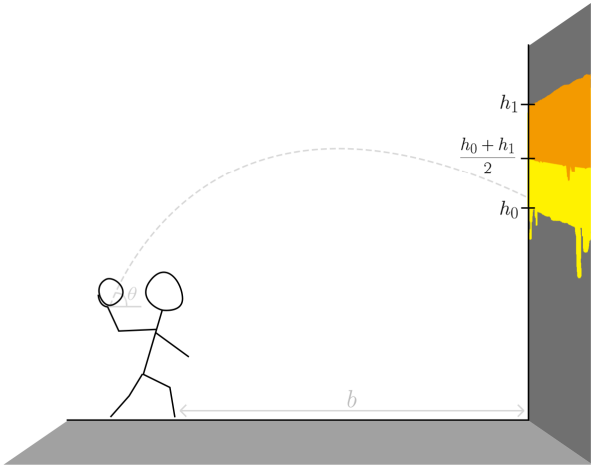
\includegraphics[keepaspectratio,alt={hit\_target}]{hit_target.png}}
\caption{hit\_target}
\end{figure}

\emph{Ilustrācija sistēmai, uz kuras pamata veidosim simulāciju.}

Bumbas augstumu var aprakstīt ar funkciju:

\[
y(t) = -\frac{1}{2} g t^2 + v_0 t + h_0,
\]

kur \(v_0\) ir sākuma ātrums, \(\theta\) ir mešanas leņķis, un
\(g = 9.81 , m/s^2\).

\begin{enumerate}
\def\labelenumi{\alph{enumi})}
\item
  Uzrakstīt funkciju, kas atgriež bumbas augstumu dotajā laikā \(t\).
\item
  Modeļa ietvaros bumba trāpīs sienai laikā
\end{enumerate}

\[
T = \frac{b}{v_0 \cos(\theta)},
\]

kur \(b\) ir attālums līdz sienai. Pēc \(y(T)\) vērtības noteiks
punktus. Punktu skaits tiek aprēķināts un atgriezts ar funkciju, kuru
jāuzraksta pašam.

Mērķis atrodas uz sienas no augstuma \(h_0\) līdz \(h_1\)
(\(h_0 < h_1\)). Punkti tiek piešķirti pēc šādiem noteikumiem:

Punkti tiek piešķirti pēc šādiem noteikumiem:

\begin{itemize}
\tightlist
\item
  Saņem 0 punktus, ja \(y(T) < h_0\) vai \(y(T) > h_1\)
\item
  Saņem 1 punktu, ja \(h_0 ≤ y(T) < 1/2 (h_1 + h_0)\)
\item
  Saņem 2 punktus, ja \(1/2 (h_1 + h_0) ≤ y(T) ≤ h_1\)
\end{itemize}

\textbf{Uzdevums}:

\begin{enumerate}
\def\labelenumi{\alph{enumi})}
\item
  Uzrakstīt programmu, kas ar for ciklu izdrukā punktu skaitu, ja
  \(h_0 = 3 , m\), \(h_1 = 3.5 , m\), \(\theta = \pi/4\),
  \(b = 3.5 , m\) un \(v_0 = 15, 16, 19, 22 , m/s\).
\item
  Uzzīmēt grafiku, kas rāda sakarību starp sākuma ātrumu \(v_0\) un
  iegūtajiem punktiem.
\end{enumerate}
